\documentclass[oribibl]{llncs2e/llncs}
\usepackage{geometry}                % See geometry.pdf to learn the layout options. There are lots.
\geometry{letterpaper}                   % ... or a4paper or a5paper or ... 
\usepackage{graphicx}
\usepackage{color}
\graphicspath{{WarpTask/figures/}{Res/figures/}} %do not forget the / at the end

\title{VLI - a library for large integer and polynomial arithemtic}
\author{Timoth\'ee Ewart\inst{1}\thanks{Acknowledgments: Maxim Milakov, Peter Messmer:   NVIDIA,   Williams Sawyer, Gilles Fourestey:  CSCS, HP2C funding, hp2c.ch}  , Andreas Hehn$^2$, Matthias Troyer\inst{2} and Thierry Giamarchi\inst{1}}

\institute{Universit\'e de Gen\`eve, \email{timothee.ewart@gmail.com}  \and Eidgen\"ossische Technische Hochschule Z\"urich }

\begin{document}
\maketitle


%%%%%%%%%%%%%%%%%%%%%%%%%%%%%%%%%%%%%%%%%%%%%%%%%%%%%%%%%%%%%%%%%%%%%%%%%%%%%%%
\begin{abstract}
We present a high-performance C++ library for high but fixed precision
(128 to 512 bit) integer arithmetic and symbolic polynomial
computations. While the large integer and polynomial computation parts
of the library can be used independently optimized kernels for symbolic
polynomials with large integer coefficients are provided. The kernels
were manually optimized in assembly language for the x86-64 and power64
architectures. Our main target application is high-temperature series
expansions which require inner products of large vectors of polynomials
with large integer coefficients. For this purpose we implemented a
tunable hybrid CPU/GPU inner product function using OpenMP and NVIDIA
CUDA with inline PTX assembly. This way we make optimal use of today's
and upcoming hybrid supercomputers and attain 67\% of the peak
performance of the current NVIDIA Kepler GPU. Compared to a pure CPU
solution using the GNU Multiple Precision Arithmetic Library (GMP) we
gain a speedup of 10x for a pure CPU inner product and 60x using a GPU
accelerator.
\end{abstract}
%%%%%%%%%%%%%%%%%%%%%%%%%%%%%%%%%%%%%%%%%%%%%%%%%%%%%%%%%%%%%%%%%%%%%%%%%%%%%%%

\section{Introduction}
\begin{itemize}
\item {\bf Why did we develop the library?}
\item Applications of large integers and polynomials in many fields of science, e.g.\ cryptography
\item our intention: special purpose library for high-temperature series expansions.
\item HTSE require symbolic polynomials with arbitrary precise coefficients. Coefficients can be represented as integers.
\item maximal integer size known beforehand
\item Hot spot of HTSE inner products of vectors of such polynomials.
\item {\bf Problems with existing libraries:}
\item GMP integers are dynamic in size and optimized to cover a large range of large integers up to several thousand bits. We need only up to 512 bits.
\item inner products of polynomials are well suited for GPUs $\rightarrow$ specialized GPU kernels required.
\end{itemize}


%%%%%%%%%%%%%%%%%%%%%%%%%%%%%%%%%%%%%%%%%%%%%%%%%%%%%%%%%%%%%%%%%%%%%%%%%%%%%%%

\section{Large integers}
\begin{itemize}
\item {\bf Description}
\item signed integer arithmetic
\item fixed size (128-512bit)
\item all standard integer operations (arithmetic, comparison and bit operations)
\item in addition to that: fused multiply-add, extended multiplication which doubles the number of bits, extended add which increases the size by one 64bit word.
\item {\bf Implementation details}
\item data is stored as 64 bit integer arrays.
\item two-complement representation
\item stack based $\rightarrow$ cheap memory allocation
\item addition and multiplication using the standard schoolbook algorithms.
\item Numbers are two small for Toom\cite{Toom} or FFT based approaches like the Sch\"onhage-Strassen algorithm\cite{Schonhage}.
\item optimized ASM kernels to use hardware features not accessible from C++ (\verb|x86_64| carry addition \verb|adcq|, 64bit multiplication \verb|mulq| which calculates low and hi 64bit part of the result.)
\item TODO which special features do we use on power64?
\item assembly code generated using \verb|BOOST_PP| to compactify the code and minimize bugs.
\end{itemize}

\section{Polynomials}
\begin{itemize}
\item {\bf Description}
\item symbolic polynomial in 1-4 variables.
\begin{equation}
    p(x,y,z,a) = \sum_{i,j,k,l} c_{ijkl} x^i y^j z^k a^l
\end{equation}
\item either ``dense'' (${i,j,k,l} \le N$) or ``triangular'' ($i+j+k+l \le N$) structure.
\item any arithmetic type as coefficient $c_{ijkl}$
\item addition, subtraction, multiplication with other polynomials and monomials
\item {\bf Implementation details}
\item structure and truncation order $N$ is compile time fixed 
\item function hooks to allow custom optimized kernels for certain coefficient types
\item The symbolic variable names are given as template parameter
\item Automatic matching of variable names of different polynomial types using template meta programming.
\end{itemize}

\section{Overview of the GPU architecture}
\begin{itemize}
\item A GPU has multiple streaming multiprocessors (SM)
\item They execute instructions in a SIMT (single-instruction, multiple-thread).
\item A group of 32 threads (called ``warp'') execute the instruction stream in a lockstep fashion on multiple data, if the threads follow different execution paths all branches need to be executed serially.
\item SM switches between up to 64 warps to hide latencies. $\rightarrow$ To gain good performance thousands of threads are necessary.
\item NVIDIA CUDA resembles this hardware properties by threads that are organized in so called blocks, which consist of a few hundred threads. A thread block is always scheduled on a single SM, but it is possible to schedule multiple thread blocks on a single SM.
\item Memory hierarchy: large (several GB) slow global memory accessible from all threads; small (a few KB) very fast shared memory which is shared among all threads of a thread block; The registers of the SM are split among all threads hosted by the SM.
\item Special purpose memories: Texture memory: globally shared, read-only, cache optimized for 2D access
\end{itemize}

\section{Optimized inner product}
\paragraph{CPU}
\begin{itemize}
\item The hot spot of HTSE are inner products of large vectors with symbolic polynomials as components. The coefficients of the polynomials are large integers.
\item We continue to use the single large integer kernels
\item OpenMP parallelization: split vector into chunks, each thread does part of the inner product
\item No SIMD, since we had to use 32bit words and the number of operations for a multiplication increases by a factor TODO due to the manual handling of the carry.
\end{itemize}
\paragraph{GPU}
\begin{itemize}
\item Many small tasks of the same form. $\rightarrow$ well suited for GPUs.
\item {\bf Implementation details}
\item Several coefficients $a_{ijkl}$, $b_{i'j'k'l'}$ of the polynomials to be multiplied contribute to the same coefficient $c_{IJKL}$ of the resulting polynomial
\begin{equation}
    c_{IJKL} = \sum_{i,j,k,l} a_{ijkl} \cdot b_{I-i,J-j,K-k,L-l}
\end{equation}
\item The number of terms in this sum depends on the orders $I,J,K,L$ of the resulting coefficient $\rightarrow$ load inbalance
\item We group 32 coefficients of the result into a task and distribute them among the warps of threads (Fig.\ \ref{fig:GPU_load_balance}). {\color{red} TODO: Tim please elaborate}
\begin{figure}[t]
    \begin{center}
    \mbox{
        \includegraphics[scale=0.37, angle=-90]{coeffs.eps} 
        \includegraphics[scale=0.37, angle=-90]{warp.eps} 
    }
    \caption{Left: Number of contributions to each coefficient of the resulting polynomial (red line) sorted in reverse order and split into tasks. Right: Load balancing of the tasks over the warps.}
    \label{fig:GPU_load_balance}
    \end{center}
\end{figure}
\item Coalesced memory access?
\item Using NVIDIA parallel thread execution (PTX) assembly language to benefit from hardware carry bit propagation \verb|addc.cc| and fused multiply add with carry bit propagation \verb|madc.cc|.
\end{itemize}
%%%%%%%%%%%%%%%%%%%%%%%%%%%%%%%%%%%%%%%%%%%%%%%%%%%%%%%%%%%%%%%%%%%%%%%%%%%%%%%

\section{Benchmarks}
\paragraph{CPU}
\begin{itemize}
\item pure CPU benchmarks were done on a Sandy bridge Intel Xeon E5-2670 with 32 logical cores.
\end{itemize}
\paragraph{GPU, hybrid}
\begin{itemize}
\item GPU benchmarks were performed on Todi, a Cray XK7 with NVIDIA Tesla K20X GPUs and AMD Opteron CPUs, at the Swiss Center for Scientific Computing (CSCS)
\end{itemize}

%%%%%%%%%%%%%%%%%%%%%%%%%%%%%%%%%%%%%%%%%%%%%%%%%%%%%%%%%%%%%%%%%%%%%%%%%%%%%%%

\section{Conclusion}
\begin{itemize}
\item We 
\item License?
\end{itemize}

%%%%%%%%%%%%%%%%%%%%%%%%%%%%%%%%%%%%%%%%%%%%%%%%%%%%%%%%%%%%%%%%%%%%%%%%%%%%%%%
\bibliographystyle{llncs2e/splncs}
\bibliography{biblio/vlibib}

\end{document}
